\chapter{Analysis of the social network \Twitter}
\label{chap:analysis}

The work wants now take a closer look at a concrete social network in order to
apply the previous described attacks on it.  Of course there are many social
networks, which can be used for harvesting data, however, the study wants to
concentrate on a big social network, which is widely used by employees and
individuals.

The requirements for the choice were, as already mentioned, a large number of
users, content, which is created by the users themselves and which is
relevant for them and an API, the prototype can use for harvesting the data.
Two big social networks fulfilled the requirements, \textit{Facebook} and \Twitter. Both are
widely used, have a large number of users, a lot of content created by the
users, and an API, which can be accessed by a \textit{REST} interface.

\textit{Facebook} however seems to be more restrictive than \Twitter{} when it
comes to allowing an application to use their API, as each application needs to
have an application key supplied by \textit{Facebook}. Furthermore, the
\textit{Facebook}
API\footnote{\url{http://wiki.developers.facebook.com/index.php/API}} is quite
big and does not support harvesting of data that much.

The \Twitter{}
API\footnote{\url{http://apiwiki.twitter.com/Twitter-API-Documentation}} on the
other side is constructed for getting and setting data, which supports the
development of a prototype. Furthermore, using the large number of messages
written by each \Twitter{} user can tell a lot more, than just using static
fields, like interests or similar. This will be showed later in this chapter.
At last, \Twitter{} was chosen due to many already existing programs and
platform bindings\footnote{\url{http://apiwiki.twitter.com/Libraries}}.

\Twitter{} is a popular social networking and micro-blogging service, that
enables users to post messages and to let other users follow those messages.
The term \textit{micro-blogging} describes a form of communication, that
consists of brief messages in text form, which then can be send over a variety
of ways, like instant messages, mobile phones, e-mail or other \cite{java2007}.

\begin{figure}[hbt]
  \centering
  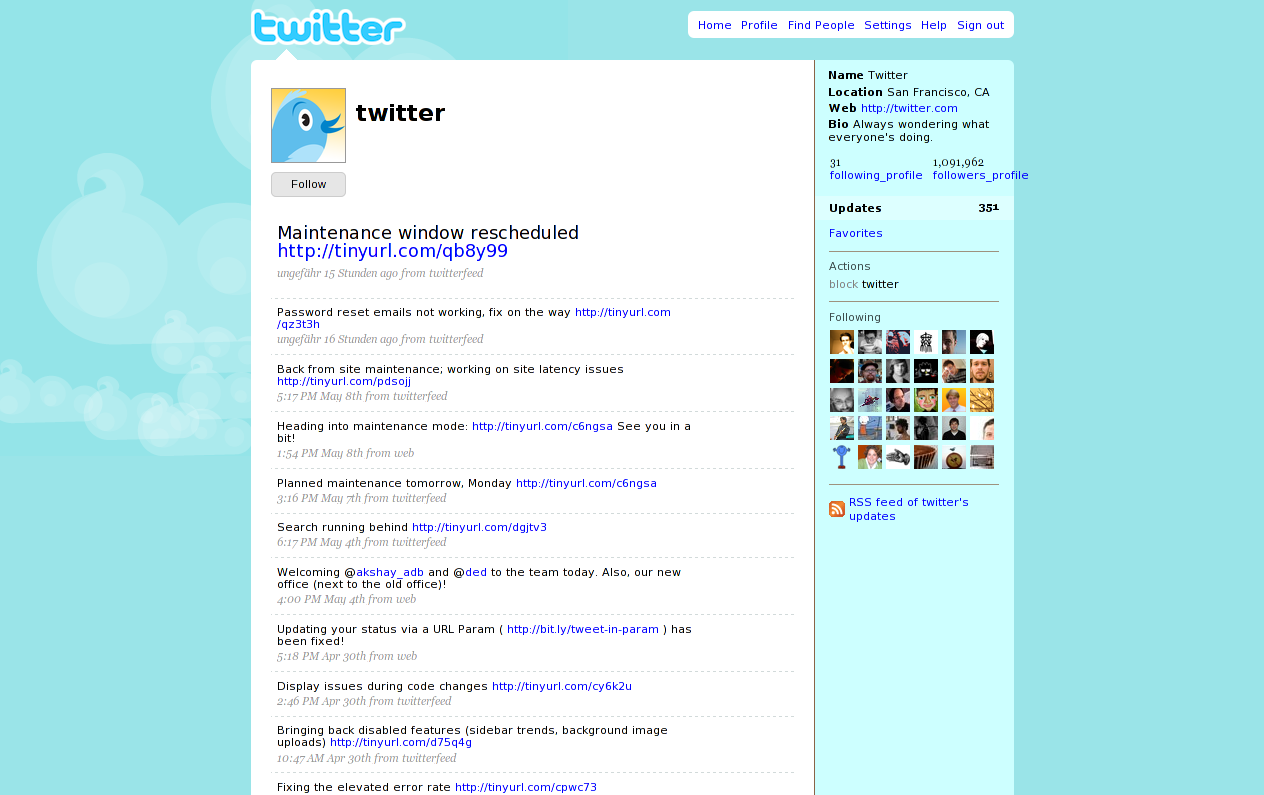
\includegraphics[width=\textwidth]{twitter_screenshot}
  \caption{An example Twitter Homepage, featuring several \Twitter{}
  messages, account information and the users this account
  follows.}\label{fig:twitter_screenshot}
\end{figure}

Micro-blogging itself is relatively new, though already widely used and
provided by services like
\textit{Twitter}\footnote{\url{http://www.twitter.com}},
\textit{identi.ca}\footnote{\url{http://identi.ca}},
\textit{Jaiku}\footnote{\url{http://www.jaiku.com}} and others. It can be
defined as a new form of communication, in which people can share short
messages by instant messaging, mobile phones, e-mail or the internet
\cite{java2007}. It is a faster way to communicate compared to other means of
communication, like blogging \cite{java2007}. It requires less time to think
and write a message, and this of course implements much quicker \textit{write
rate}. This is of course one of the main differences between blogging and
micro-blogging, whereas an author spends several minutes to hours to think up
and write a blog post. As it now takes less time to think and write a message,
the frequency one can write such, increases and a micro-blogger may posts
several messages a day.

\Twitter{} is one of the most popular micro-blogging services \cite{java2007}
and currently exhibiting more than a million users. The accurate number
unfortunately is not available, however there were estimated about 1.4 million
users in 2008 \cite{krishnamurthy2008} and more than 1.78 million users in
2009 \cite{whitworth2009}.

The social network limits the length of the messages to 140 characters. The messages
are called \textit{updates} or \textit{tweets}. The scopes of those messages
range from events, news, daily life and other interests \cite{java2007}. Of
course, other services like instant messaging also offers a way to communicate
the such informations, however micro-blogging allows to do this publicly.

Users may choose to make their messages visible to all users (even those not
logged into \Twitter{}) or to just make them available to \textit{friends}. A
\textit{friend} is a relation inside the \Twitter{} platform, and allows a user
to \textit{follow} the messages from other members, who are added as a
\textit{friend}. Users, who are not a friend to another user can still follow
the user, who they are not friend with, but are then called \textit{follower}.
The friend relation is not forced to be mutual, but can be single-way too. In
addition, a user can choose to make his messages public or just available to
his friends. If the messages are marked as public, they will be displayed in
the public timeline, which can be accessed by the URL
\url{http://twitter.com/public_timeline}.

The main types of user interactions are daily chatter, conversations, sharing
informations and reporting news \cite{java2007}. This of course leads us to
question, which information can be dangerous and which can be used by a social
engineer.

\begin{figure}[hbt]
  \centering
  \begin{tikzpicture}[scale=0.75, transform shape,
                      root concept/.append style={concept color=skyblue1},
                      level 1 concept/.append style={concept color=chameleon2},
                      text=white, mindmap]

    \tikzstyle{every annotation}=[fill=skyblue3, font=\sf]

    \node[concept] (Twitter) {Twitter}
      child[concept, grow=160] {node [concept] {Web Interface}}
      child[concept, grow=125] {node [concept] {Twitter API}
      child[concept, grow=left] {node [concept] {User Applications}}}
      child[concept, grow=90] {node [concept] {Facebook}}
      child[concept, grow=55] {node [concept] {IM}}
      child[concept, grow=20] {node [concept] {SMS}}
      %
      child[concept, grow=200] {node [concept] {Web Interface}}
      child[concept, grow=235] {node [concept] {Twitter API}
      child[concept, grow=170] {node [concept] {RSS}}
      child[concept, grow=210] {node [concept] {User Applications}}}
      child[concept, grow=270] {node [concept] {Facebook}}
      child[concept, grow=305] {node [concept] {IM}}
      child[concept, grow=340] {node [concept] {SMS}};

    \node[annotation] at (52.5:7.5) {Twitter Input Methods};
    \node[annotation] at (307.5:7.5) {Twitter Output Methods};

    \draw (2,0) -- (6,0);
    \draw (-2,0) -- (-6,0);

  \end{tikzpicture}
  \caption{\Twitter{} input and output methods, on the basis of \cite{krishnamurthy2008}.}
  \label{fig:twitter_io}
\end{figure}

A sample \Twitter{} profile page is shown in figure
\ref{fig:twitter_screenshot}. It features several elements, which we will
discuss in the next section. 

\Twitter{} messages can be sent and received by a variety of methods, all
listed in figure \ref{fig:twitter_io}. Several of those are or were
discontinued for a certain amount of time, but either re-enabled or provided by
a third party company.

\section{\Twitter{} profile data}
\label{sec:twitter_profile_data}

As already mentioned, a \Twitter{} profile page consists of a series of
elements, which can be used for harvesting data. The complete profile data,
which can be accessed is described in appendix
\ref{chap:twitter_profile_data}. Relating to a social engineering attack,
not all elements are needed. However, those needed, are described in section
\ref{sec:relevant_data}.

\section{Message classification}

In order to see, what and how messages can be useful for an attack, a social
engineer might be interested in a classification of the messages of the victim.
Java et al. describe a classification of the messages on the \Twitter{}
platform \cite{java2007}. After they gained a dataset, the author and his team
tried to categorize each message. The results were the following:

\begin{description}

\item[Daily Chatter]
Most users on \Twitter{} post about what they are currently doing or similar
things. Of course, they are answering the question \flqq{}What are you
doing?\frqq{}, which can be found over the input field of a message. This is
the most common use of the \Twitter{} platform.

\item[Conversations]
There are two ways to communicate with another user, one is by public
messaging, which features the @ symbol like stated above, the other one is
private messaging, which uses the D character. About one eighth of all posts
in their dataset contained a public conversation and about 21\% of the users in
their dataset used this type of messaging \cite{java2007}. Of course, there is
no data available about private messages.

\item[Reporting news]
Another big piece of the cake is done by users, who report or comment news and
events. Some of them are automated and post weather reports, other are
eyewitnesses and report and event in their location.

\item[Sharing information/URLs]
Many users also share information and websites, and therefore uses services,
like \textit{TinyURL}\footnote{\url{http://tinyurl.com/}} or
\textit{tr.im}\footnote{\url{http://tr.im/}}. According to Java et al.,
about 13\% of all posts in the dataset contain at least one URL \cite{java2007}.

\end{description}


\section{Relevant data and the security risks of those at individuals and companies}
\label{sec:relevant_data}

\subsection{The challenge of extracting data automatically}

The \Twitter{} social network gives access to a \textit{REST} API, which can be
used by calling either \url{twitter.com} or \url{search.twitter.com}. The first
one is used for account settings and methods, posting updates and several other
things related to users, their relationship and updates. The latter one is used
for searching for certain updates of users or users themselves. The API
supports \textit{JSON}, \textit{XML}, \textit{RSS} and \textit{Atom} as output
formats, allthough just \textit{JSON} is supported on every API method.

Most API methods require a username and a password, however this is not a
problem by itself, as a \Twitter{} account can be created within minutes by
using an e-mail address. The real challenge however is the limit of 150 API calls
per hour. If a user is logged in, the user has 150 calls, which he can use on
API calls. If the user is not logged in, i.e. an anonymous user, the IP address
is used for tracking this user. To make use of a very deep information
visualisation of a user, 150 calls are not enough, as for example many users
have more than 150 friends. However, there are three ways around this problem:
The first one is to just use the important data, leaving a deep information
visualisation of e.g. friends aside, the second is to create many accounts, and
then change the accounts during acquiring the data, and the last one to not log
in into \Twitter{} and acquiring the data anonymously, while changing the IP
address after 150 calls. However, some API methods require the user to be
logged in. A compromise between these methods might be the best possibility,
e.g. acquiring as much data as possible about a single user and then repeat the
same for several other users, who are in contact with him and might be
interesting for an attack.

\subsection{Ontology and classification of the data}

The \Twitter{} API offers a wide range of methods, admittedly in the first place,
the attacker is mostly interested in gaining information and not that much in
using the API methods to do actions. Additionally the attacker is mostly
interested in a certain person or group, therefore just the methods, which
allow gathering data about a certain user or group makes sense here. For a
social engineering attack, the following data might be interesting.

\begin{figure}[hbt]
  \centering
  \begin{tikzpicture}[scale=0.75, transform shape,
                      root concept/.append style={concept color=skyblue1},
%                      level 1 concept/.append style={concept color=chameleon2},
                      text=white, mindmap]

    \tikzstyle{level 2 concept}+=[sibling angle=45]

    \path[mindmap]
      node[concept] {User}
      child[concept color=scarletred1, grow=0] {
        node[concept] {Friends}
        [clockwise from=90]
        child { node[concept] {Replies} }
        child { node[concept] {Shared Interests} }
        child { node[concept] {Friends} }
        child { node[concept] {Colleagues} }
        child { node[concept] {Followers} }
      }
      child[concept color=butter2, grow=90] {
        node[concept] at (90:1) {General data}
        [clockwise from=112.5]
        child { node[concept] {Name/ Username} }
        child { node[concept] {Personal description} }
        child { node[concept] {Homepage} }
        child { node[concept] {Picture} }
        child { node[concept] {Time Zone} }
        child { node[concept] {Location} }
        child { node[concept] {Profile creation date} }
        child { node[concept] {Messages} }
      }
      child[concept color=chameleon2, grow=180] {
        node[concept] {Messages} 
        [clockwise from=295]
        child { node[concept] {E-mail addresses} }
        child { node[concept] {Times} }
        child { node[concept] {Replies} }
        child { node[concept] {Input sources} }
        child { node[concept] {Interests} }
        child { node[concept] {Locations} }
      };
  \end{tikzpicture}

  \caption{Graphical representation of the data classification.}
  \label{fig:twitter_ontology}
\end{figure}


\subsubsection{General data about the user}
\label{sssec:general_data}
\Twitter{} offers some static fields, which can be altered by the user and
remains mostly the same over the year. Some other information is created
automatically and still accessible by other users.

Most of the fields described in appendix \ref{chap:twitter_profile_data} are
already usable for gaining an already penetrative overview of a person.

\begin{description}
\item[Name] Gives the real name of the user, which can be used for
phishing mails or social engineering attacks, where a name is needed.

\item[Username] Many users use the same username on different
services, like e-mail or other social services. This can be used for some
attacks.

\item[Description] This description might be useful for gathering other useful
information, such as workplace or interests.

\item[Homepage] A personal homepage might give additional
information about the user.

\item[Picture] Gives an idea, how the person might
look like.

\item[Time Zone] Gives an idea, where the person
lives or works.

\item[Location] Together with the Time Zone, an attacker now
could actually define his work place and home more precise.

\item[Profile Creation date] Tells the attacker
since when the user is using \Twitter{}. That might be a good indication,
whether he also uses other services and since when.

\item[Messages] The Message count could tell how active a person using a
computer or how interested he is in a certain topic.

\item[Followers] An interpretation of the followers count may say how
famous he is and how much effect he could have on other people.

\item[Friends] While the number of friends is not that interesting,
the friends can be used for attacks too, as most of them are real friends
or colleagues.
\end{description}

\subsubsection{E-mail addresses}

As already described earlier, the e-mail addresses of the users are not visible
throughout \Twitter{}, though the addresses can be gathered in most cases.
Brown et al. for example described, that an e-mail address can be constructed out
of a naming scheme of given data, like the username or the real name
\cite{brown2008}. Another possibility is to look through the messages for
anything that looks like an e-mail address. Quite often users write messages,
about contacting them at a special address or that they changed to a new one.

\subsubsection{Times}

An analysis of the time of writing messages can be a good instrument to track
down working hours and working days or periods the user is using a computer.
Additionally hours, the user is not available can be tracked too, for example
when the user is doing holidays.

\subsubsection{Replies and friends}

\Twitter{} by itself does not publish the friends of a user, however it
promotes followers and users who follow the candidate. With this data however,
the \textit{hidden} network can be found, which basically is a graph, which
only consists of bidirectional connections. This is the network, the user is
actually friend with. By analysing the replies of messages, it can be found,
with which of the friends, the user has most contact with. This shows then a
quite good representation of the users friends and or colleagues.

\subsubsection{Input sources}

The \Twitter{} input sources give an overview, what methods the user uses to
post updates. For example, if he is using a \Twitter{} client, that is only
available for a certain operating system, this could be exploited. If the
source is mostly SMS, the location is getting even more important, as location
tracking could be done in this case. Also there could be a relation between the
input method and the computer experience the user has, if he is using external
clients or not.

\subsubsection{Interests}

In most messages, the users represent a certain interest in a single topic.
This is either done by marking the topic explicitly with a hash sign or by just
using text to describe the interest. 

\subsubsection{Locations}

Also, many messages include information about the current location, for example
if they arrive at the workplace, at conferences or other. This data can be
filtered by analysing the messages. A promising project, that could be used
here is \textit{TwitterData}\footnote{\url{http://twitterdata.org/}}, which
marks keywords as key value pairs and actually promotes keys like
\textit{location}, \textit{lat} and \textit{long} for location, latitude and longitude
positions.

\subsubsection{Text search}

Finally a text search can be used to get further information about a certain
topic the user wrote about. 

\section{Threats and risks}

All of the above mentioned fields and data, create a threat to the user himself
and also to other users, who are in contact with him. The threat and risk does
not directly come from the information gained, but from the fact, that every
piece of information a social engineer can bring together, builds an even
better base or starting point for a social engineering attack
\cite{mitnick2003}. This means, that the information itself, does not create a
threat, however, the social engineering attack does.  Even with at first glance
useless information, an attack can be driven. For example, if a user shares his
location and what he is doing job-wise, his workplace and position can be
easily found.

There are various scenarios, which are possible using different data. As it is
possible to create a quite expletive ontology about a person just with the
fields and data mentioned above, further attacks are supposable.

Another matter is the almost hidden information retrieval possibility. If a
social engineer has to create a contact to his victim or to other persons, who
are in contact with the victim over the telephone or e-mail, the attacker could
be detected. In this scenario however, only the provider of the social network
tracks the information retrieval. If the attacker now does not stand out in
relation to other retrievals, as normal clients, which are accessing the social
network, there is probably no way to detect the attacker. This is a very vital
matter for a successful social engineering attack.

The prototype, which is described in the next chapter, will make
use of exposed data, building a fact sheet about the user and people, who are
in contact with. This is then used to create a social engineering attack,
showing that such attacks basing on data of social networks are already
possible.

\section{Countermeasures}

The nature of a social network, especially \Twitter{} is sharing data.
Therefore it is difficult to encounter attacks and there has to be a trade-off
between utility and security \cite{brown2008}. Given also, that most data comes
out of analysing the messages, there are not many ways to exclude the risk.
However, there are various methods to minimize the likeliness of a social
engineering attack, based on the data published on \Twitter{}.

\subsection{Preventions by the user}
\comment{better title needed}

The first way to minimize the risk, would be to protect the updates, which
basically means, that only users, who are approved by the author of the updates
may see them. This however lacks in two facts, first the fields described in
section \ref{sssec:general_data} are still visible. Second, the attacker could
just become a friend with the victim and gain access to the messages.

Another, possibly extreme, way would be to not publish sensitive information
about the user himself, his workplace, friends and other.

This is of course quite hard to accomplish, as the whole idea about \Twitter{}
is to share information. Even, if a user would accomplish this, lots of
information would be still easily accessible, like the times analysis, his
friends, colleagues and much more.

At last, a user could not use a social network like \Twitter{}. This certainly
would exclude the chance of being a victim in a social engineering attack,
based on the data found on \Twitter{}. However, if this solution is suitable
for everybody, should be left to one's own devices.

\subsection{Preventions by \Twitter{}}
\comment{better title needed}

Having a look on the whole social network, there are not many solutions, in
which \Twitter{} could minimize the risk either.

One possibility would be to require each user to be logged in to view the
messages of other users. This however would detach the \Twitter{} social
network from the outside and probably not the right way for a commercial
oriented company. Anyhow, if that would be the case, an account could be easily
made and so there won't be any surplus.

At last, the social network could limit the API calls and track them more
precise, so that an automatic extraction is no more possible or at least made
harder. But to decide, which data is harmless and which could be used for an
attack is very difficult, as both fetch almost the same data. The only
difference could be the fact, that an attacker is interested more into a single
user, while an unoffending \Twitter{} client might be more interested in many
users. Although, if there would be a way to accomplish this, it would be
probably the only countermeasure, which really would hinder an attacker of
gaining information.
